\documentclass[pdflatex,sn-basic,Numbered]{sn-jnl}

\usepackage{graphicx}
\usepackage{multirow}
\usepackage{amsmath,amssymb,amsfonts}
\usepackage{amsthm}
\usepackage{mathrsfs}
\usepackage[title]{appendix}
\usepackage{xcolor}
\usepackage{textcomp}
\usepackage{manyfoot}
\usepackage{booktabs}
\usepackage{algorithm}
\usepackage{algorithmicx}
\usepackage{algpseudocode}
\usepackage{listings}

\raggedbottom

\begin{document}

\title[Unsupervised Functional Stage Detection From EEG Using Topological Data Analysis]{Unsupervised Functional Stage Detection From EEG Using Topological Data Analysis}

\author*[1]{\fnm{Aleksandr} \sur{Abramov}}\email{asabramov@edu.hse.ru}
\author[1]{\fnm{Ekaterina} \sur{Mikhaylets}}
\author[2]{\fnm{Vsevolod} \sur{Chernyshev}}
\author[3]{\fnm{Alexander} \sur{Kaplan}}
\author[1]{\fnm{Fedor} \sur{Ratnikov}}

\affil[1]{\orgdiv{Faculty of Computer Science}, \orgname{HSE University}, \orgaddress{\state{Moscow}, \country{Russia}}}
\affil[2]{\orgname{Ulm University}, \orgaddress{\state{Ulm}, \country{Germany}}}
\affil[3]{\orgname{Lomonosov Moscow State University}, \orgaddress{\state{Moscow}, \country{Russia}}}

\abstract{Electroencephalogram (EEG) segmentation is primarily a manual, routine task performed exclusively by specialists. Recent studies have proposed the state-detecting algorithm (SDA) --- an automated technique for detecting functional stages with minimal human intervention --- which has proven effective using spectral features. This paper introduces an alternative feature engineering approach aimed at exploring the spatial structure of data using the emerging field of topological data analysis (TDA). We propose an algorithm to extract a comprehensive topological description of EEG with several thousand features and suggest QSDA, a feature selection framework based on SDA performance. Next, we apply the procedure to the EEG recordings from two different domains and observe well-separated stage boundaries in all cases, suggesting that TDA complements or even supercedes the spectral features and reveals new, previously unknown patterns. Moreover, we obtained good quality with noisy data and poor results with shuffled epochs, confirming the robustness of the technique. Overall, the algorithm proved to be a viable feature engineering approach for SDA, indicating the existence of significant patterns in the spatial structure of EEG signals, which may have interesting physiological interpretations leading to more effective and robust functional stage detection.}

\keywords{topological data analysis, state-detecting algorithm, functional states, feature selection}

\maketitle

\section{Introduction}

Electroencephalograms (EEG) are a powerful tool for studying human brain activity and diagnosing numerous diseases and abnormalities. However, its analysis is usually performed manually, and automation in the field is vastly limited to specific tasks. Most algorithms rely on information about events artificially created during the experiment (external interactions with the subject, reactions, responses, etc.). Currently, the study of EEG of continuous processes that do not allow external interactions with the subject is of significant value for neurophysiology, including somnology and epilepsy detection.

One such task is to find the boundaries of functional states in the EEG that split the recording into well-separable parts, denoting the occurrence of some naturally induced events. To solve this problem,~\cite{SDA} recently presented the state-detecting algorithm (SDA), which operates without any additional information about the events that occurred during the experiment (including their exact amount) using traditional data clustering methods. The technique consists of two principal stages: finding the potential boundaries of functional states for different values of hyperparameters using hierarchical clustering with a connectivity constraint, and applying another suitable clustering to those answer sets to deduce the resulting boundaries based on the final quality metrics.

To use the algorithm, one should clean and preprocess the EEG data, split it into epochs, and embed the corresponding time series into some feature space. As shown in the original work, the method demonstrates good quality for EEG obtained from the Tantric Guhyasamaja meditation of Buddhist monks using traditional spectral features to describe the time series: PSD, PLV, and Coherence.

However, these features mostly describe the frequencies and correlations in the time series, leaving significant portions of the information unexplored. Currently, there is ongoing research on the applications of another modern approach to feature extraction --- topological data analysis (TDA), which identifies the relationships in the data by studying its geometry and spatial structure via the research of the appearance and disappearance of holes and voids in the data across dimensions. It allows for the quantification of different structural characteristics of the signal, which are known to be more convenient for some problems, including in physiology, can achieve better quality, and the results may be relatively easy to interpret.

Numerous recent studies have shown that TDA demonstrates high quality in solving various problems, including time series and EEG in particular. For example,~\cite{chazal2024topologicalanalysisdetectinganomalies,rai2024identifyingextremeeventsstock,heo2024persistenthomologyfeaturedtime,chrétien2024timetopologicalanalysiseeg} presented numerous theoretically guaranteed approaches to detecting anomalies in multivariate time series, demonstrating their quality with diverse datasets ranging from synthetic, generated ones to real-world examples, including the stock market, music recordings, and epilepsy detection.~\cite{dimontesano2024dynamicallymaintainingpersistenthomology} proposed a data structure to maintain and recalculate the persistent homology as epochs are added to or removed from the time series, and~\cite{ost2024bananatreespersistencetime} elaborated on the real-world applications of the technique.~\cite{cai2024topologicalfeaturesearchmethod} demonstrated the application of TDA in ADHD classification, achieving exceptional results for typical datasets in the field with high precision and robustness. Finally,~\cite{deng2024twostagehierarchicalexplainablefeature} suggested a TDA-based feature selection framework to improve the performance of dimensionality reduction in sleep stage classification.

In this study, we apply topological data analysis to find functional states in the EEG of continuous processes --- the aforementioned Tantric Guhyasamaja meditation practice and the whole-night polysomnographic (PSG) sleep. To evaluate the applicability of the approach to the problem, we propose a framework for calculating a comprehensive description of several thousand features describing various aspects of the time series using diverse topological methods and statistical characteristics. We then present QSDA, an SDA-based feature selection technique to select a reasonable number of features that achieve the best quality of the final answer. We show that the approach is efficient in filtering out the least valuable features and can noticebly improve the final results. Finally, we compare the obtained state boundaries computed by SDA with expert annotations for sleep data and with results obtained using different feature sets and data modifications for meditation data, and draw conclusions based on the output's quality metrics. Additionally, we utilize information value analysis to estimate the influence of individual features on the answer, confirm the stability of our feature selection algorithm, and reinforce the obtained results.

\section{Methods}

\subsection{Datasets}

\subsubsection{Meditation data}

Guhyasamaja Tantra is a traditional meditation practice that follows the strict principles enshrined in the sacred scriptures of Buddhism. Its essential part consists of eight subsequent stages, the durations of which may vary in different versions.

The data used in the study are EEG recordings of the successful meditation of 30 Tibetan Buddhist monks practicing Guhyasamaja Tantra for many decades. The dataset was collected during three expeditions, each of which yielded recordings from 12, 14, and 4 monks, respectively. The signals were acquired using an NVX-52 system at a 500 Hz sampling rate with analog bandpass filtering from 0.1 to 200 Hz and a digital notch filter at 50 Hz to remove power line noise. The first three recordings have been presented in the original paper~\cite{SDA}, and are thus of the most interest in this work. 

Several procedures, including a bandpass filter at 0.9 -- 40 Hz and independent component analysis, were applied to remove artifacts unrelated to the process of interest (respiratory and muscle activity, eye blinking, heartbeat, etc.). The recordings were then divided into 1-second epochs, 10 -- 15\% of which, most deviating from the average by the power spectral density, were removed. No overlap was used when creating the epochs, except for subject 1, which used an overlap of 0.2 seconds. The resulting data are arrays of epochs, where each epoch is a multidimensional time series represented with a matrix, with each channel corresponding to one electrode used during the experiment.

Since the recordings were obtained during separate expeditions, the data includes three groups of EEG with slightly different electrode sets. The first expedition (12 recordings) used 38 electrodes, while the second (14 recordings) and third (4 recordings) utilized only 32, differing in the placement of AF1, AF2, F3, and F4. In all cases, the ear electrodes were excluded from the research, as their data primarily describe muscular activity, which is not relevant to the study. For ease of analysis, as in the original paper, we divided the electrodes into 11 regions of interest based on the brain parts they recorded, as shown in Supplementary Materials A.

\subsubsection{Sleep data}

To validate the approach and assess its general applicability, we utilized sleep-edf~\cite{SleepEdf,PhysioNet} --- a more common, public dataset of 197 whole-night polysomnographic sleep recordings. It contains two subsets: 153 recordings from the Sleep Cassette Study (SC) and 44 recordings from the Sleep Telemetry Study (ST). In this work, we focus on the former group collected from people without any known sleep disorders.

The data were obtained during a 1987 -- 1991 study of age effects on sleep involving 77 subjects aged between 25 and 101. In this study, though, we discard any additional information about the subjects, including their age and sex, and focus on the PSG recordings themselves. The signals contain three EEG channels, one EOG channel, chin EMG, body temperature, and a respiration monitoring channel. For each recording, the dataset also provides stage annotations from well-trained experts. To speed up the computations, we resample all channels from 100 Hz to 50 Hz, crop the data to a maximum of 15 minutes of wake time at the beginning and end of the recording, and split it into 15-second epochs without overlapping. To simplify the analysis, we also discard the segments with unknown labels, combine stages N3 and N4, and predict at most 10 sleep stages for each subject to compare them with the best-fit subset of 10 stages from the target annotation.


\subsection{State-Detecting algorithm}

The State-Detecting algorithm is a novel data-driven approach for finding the functional states in the EEG from its feature description --- a matrix that maps each epoch to a feature vector of a given dimension. The technique combines two clustering methods to find the resulting edges, accounting for the continuity of the process under analysis in time. Here, we briefly review the general principles of both stages. Please refer to the original study~\cite{SDA} for a more detailed description.

In the first step, the algorithm finds the potential boundaries of functional states using Ward's hierarchical clustering method with different values for the number of sought stages and the maximum time between epochs in the connectivity matrix. The obtained boundaries are then sorted, and the neighboring stages are merged if they are too short or do not differ sufficiently by the Ward distance.

In the second step, the algorithm utilizes K-Means to select the candidates for the final boundaries of functional states based on the results of the first step. For this, the SDA applies the aforementioned clustering method to the joint sets of potential boundaries obtained previously to determine the required number of stages. Finally, the algorithm computes the resulting boundaries as modes and medians of the obtained clusters merged similarly to the first stage to guarantee their sufficient length and dissimilarity.

The conclusive answer is decided by an expert decision accounting for the clustering quality metrics. In this study, we primarily focus on the silhouette score that is calculated for one object using equation~\eqref{eq1} and shows the similarity of this object to other objects in its cluster ($C_x$) in comparison with objects in different clusters ($C_y$). The single value for the entire set is obtained by averaging the results across all studied objects. The metric ranges from -1 to 1, where positive values indicate that the object is assigned to the correct cluster, which is well separated from other clusters. To account for the continuity of the studied process in time, we use a so-called adapted silhouette score computed as the average silhouette score of all pairs of clusters that are adjacent in time, since the EEG may contain multiple instances of the same stage that cannot be merged as they are separated by another stage.
\begin{align}
    a(x, C_x) = {(|C_x| - 1)} ^ {-1} \sum_{y \in C_x} ||x - y||, \nonumber\\
    b(x, C_x) = \min_{C_y \ne C_x} {|C_y|} ^ {-1} \sum_{y \in C_y} ||x - y||, \nonumber\\
    s(x, C_x) = (b - a)~~/~~\max(a, b) \label{eq1}
\end{align}


\subsection{Topological data analysis}

Topological data analysis is a modern approach to analyzing different data by studying their spatial characteristics (shape, structure, etc.) using algebraic topology. The main tools of this approach are persistent homologies and persistence diagrams, calculated for metric spaces to describe the number and stability of multidimensional `holes' in them. It has been shown that minor perturbations in the source data do not significantly affect the results, making it possible to use the information from the diagrams to solve various machine learning problems according to the following general principle.

First, transform the input data into a metric space --- a set of points with a correctly defined distance function. In this study, we utilized two principal approaches: the Takens' embedding algorithm~\cite{10.1007/BFb0091924,perea2013slidingwindowspersistenceapplication} to explore individual components of the time series and the Pearson dissimilarity to investigate correlations between them. For the former, the general hyperparameter selection methods (that is, the dimensionality of the embeddings~\cite{PhysRevA.45.3403} and the time delays between them~\cite{PhysRevA.33.1134}) aim to optimize the mutual information and the number of false-neighboring pairs of points. For the latter, we define the distances between the components of a multivariate time series as their Pearson dissimilarity, thus obtaining a point cloud.

Second, construct a sequence of nested simplicial complexes --- topological spaces homotopy equivalent to the unions of balls of a given radius around the points from a given set for all positive values of the filtration parameter. However, due to excessive computational costs, in practice, an approximation called the Vietoris--Rips complex~\cite{Vietoris1927} is typically utilized. The structure represents unions of simple geometric figures of various dimensions (segments, triangles, tetrahedra, etc.), called simplices, for which all pairwise distances between vertices are less than $\epsilon$. The general algorithm for constructing a filtration is to observe the appearance and disappearance of simplexes with increasing values of $\epsilon$, although several more efficient algorithms have been proposed (e.g. \cite{Bauer_2021}).

Next, calculate the persistent homology of the resulting structure based on the `moments' of appearance and disappearance of simplices. Construct and filter (that is, remove the points closest to the diagonal, which carry little information and most likely describe the `noise' in the data) the persistence diagram, where each simplex corresponds to one point with coordinates representing the moments of its appearance in and disappearance from the complex, respectively.

Subsequently, extract the features --- various topological and statistical characteristics --- from the persistence diagram. The principal approach studies Betti numbers~\cite{Zomorodian2005}, which represent the maximum number of cuts before separating the surface into two parts. Multiple other techniques have been proposed, including the persistence entropy~\cite{10.1007/978-3-319-29228-1_11}, landscape~\cite{bubenik2015statisticaltopologicaldataanalysis}, silhouette~\cite{chazal2013stochasticconvergencepersistencelandscapes}, and amplitude. The latter is particularly interesting as a measure of the difference between a given persistence diagram and an `empty' diagram, computed based on other topological characteristics as well as methods from adjacent fields of study, such as the Wasserstein and bottleneck distances~\cite{Efrat2001}.

Finally, select the most valuable features and reduce their dimensionality to remove noise and improve the quality of subsequent machine learning algorithms. For the latter, we used principal component analysis (PCA), which is a typical method that has demonstrated reliability and good performance in many previous studies. As in the original paper, the technique was applied with 15 components, a robust choice with a good balance between preserving variance and filtering noise, as we also confirm experimentally.

\subsection{Feature engineering}

As shown in Fig. \ref{figure1}, we employ three independent techniques to extract features from the EEG.\@

\begin{figure}
    \centering
    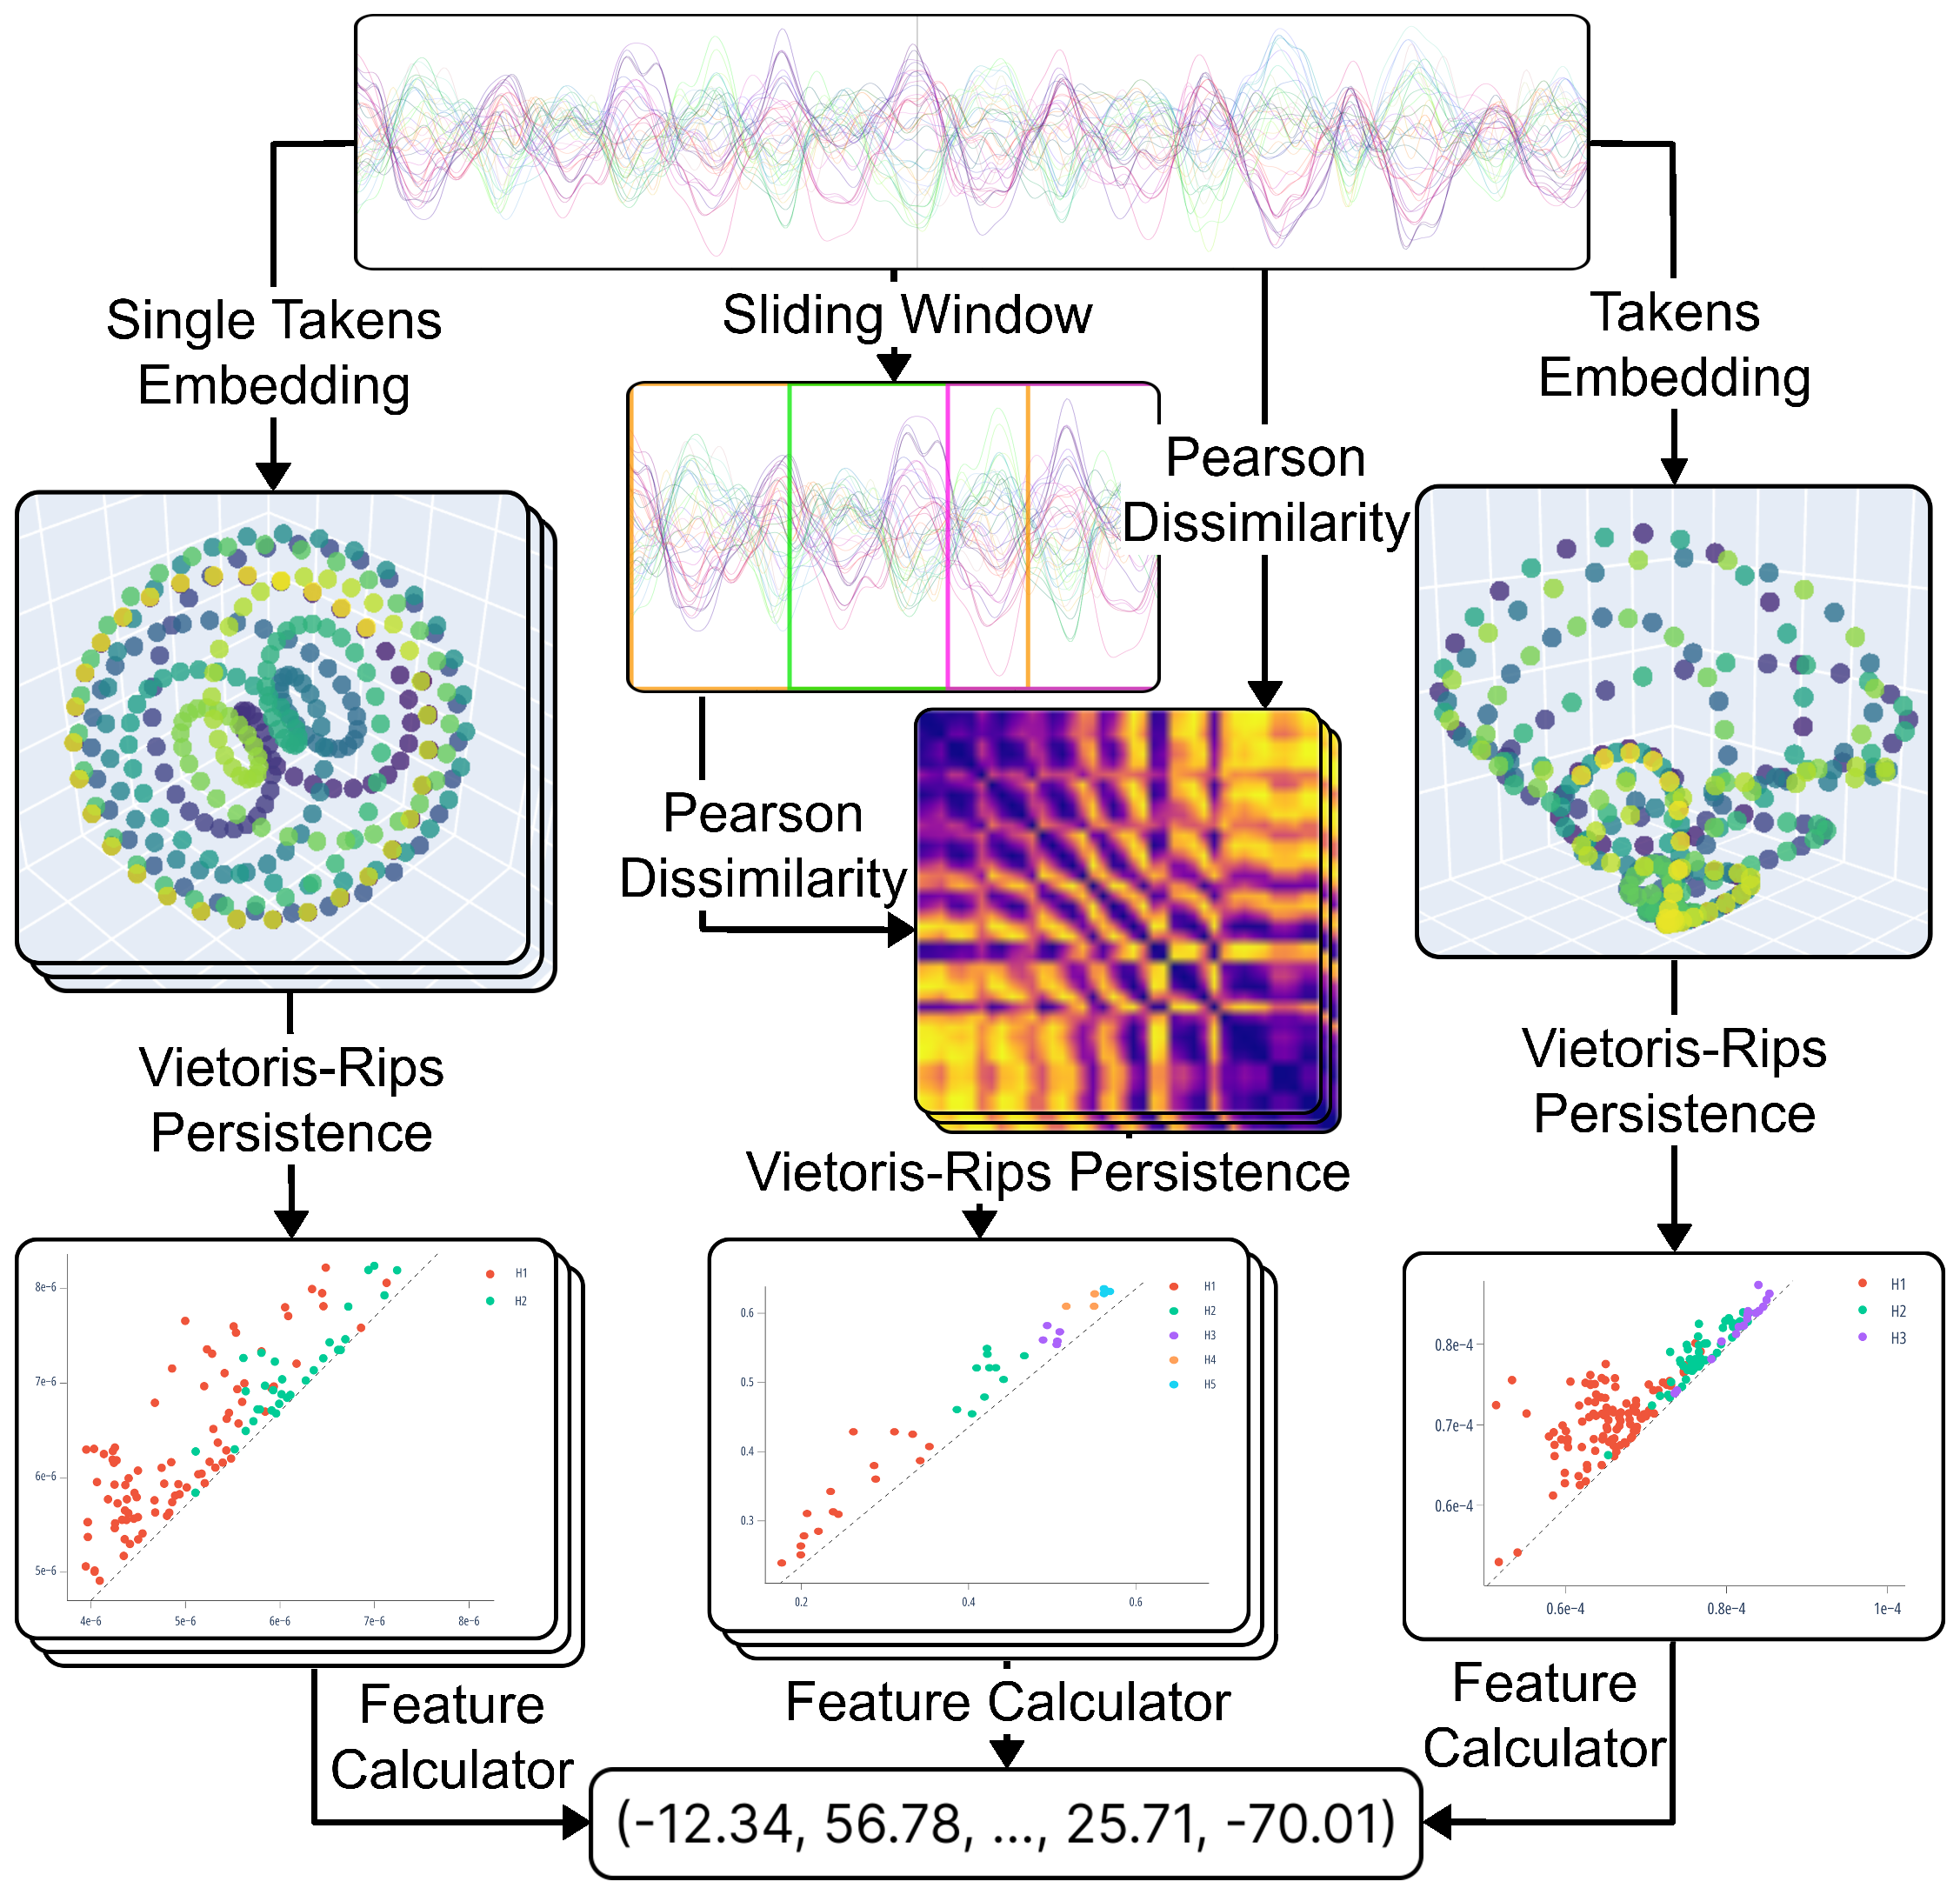
\includegraphics[width=0.5 \columnwidth]{new_Fig1.eps}
    \caption{The algorithm for extracting topological features from the EEG\@}
    \label{figure1}
\end{figure}

First, the components are processed independently to analyze the data obtained at each electrode separately from other parameters. For this, we divide the epochs --- multidimensional time series --- into sets of one-dimensional time series, each corresponding to one electrode during the experiment. Then, we calculate the optimal hyperparameters of the Takens embedding algorithm, acquiring a set of values for each epoch of each EEG component. Finally, we select one value for each that is optimal for most epochs, transform the original data into metric spaces using the Takens algorithm with those best hyperparameters, construct Vietoris--Rips complexes, and compute persistence diagrams.

This approach describes individual EEG variables and detects most of the significant patterns in the data. However, it does not account for correlations between the components, which may also contain valuable information.

To address this issue, the second approach aims to analyze the relationships between the EEG components. The point clouds are obtained by calculating the Pearson dissimilarities between the channels for each epoch and all its sliding windows of a given size with a fixed step. The result is a set of matrices describing metric spaces consisting of as many points as the number of channels in the data, with distances reflecting the correlations between the corresponding components. Then, similar to other techniques, we construct Vietoris--Rips complexes to produce persistence diagrams and obtain the feature descriptions of the EEG.\@

Eventually, we analyze the time series as a whole without explicitly focusing on specific characteristics. To do this, we employ the multidimensional Takens algorithm with hyperparameters determined experimentally but kept identical for all components. The retrieved metric spaces are again processed with Vietoris--Rips complexes to obtain the resulting features.

\subsubsection{Extracting features from persistence diagrams}

To vectorize the persistence diagrams as part of the feature engineering process, we implemented the pipeline in Fig. \ref{figure2}.

\begin{figure}
    \centering
    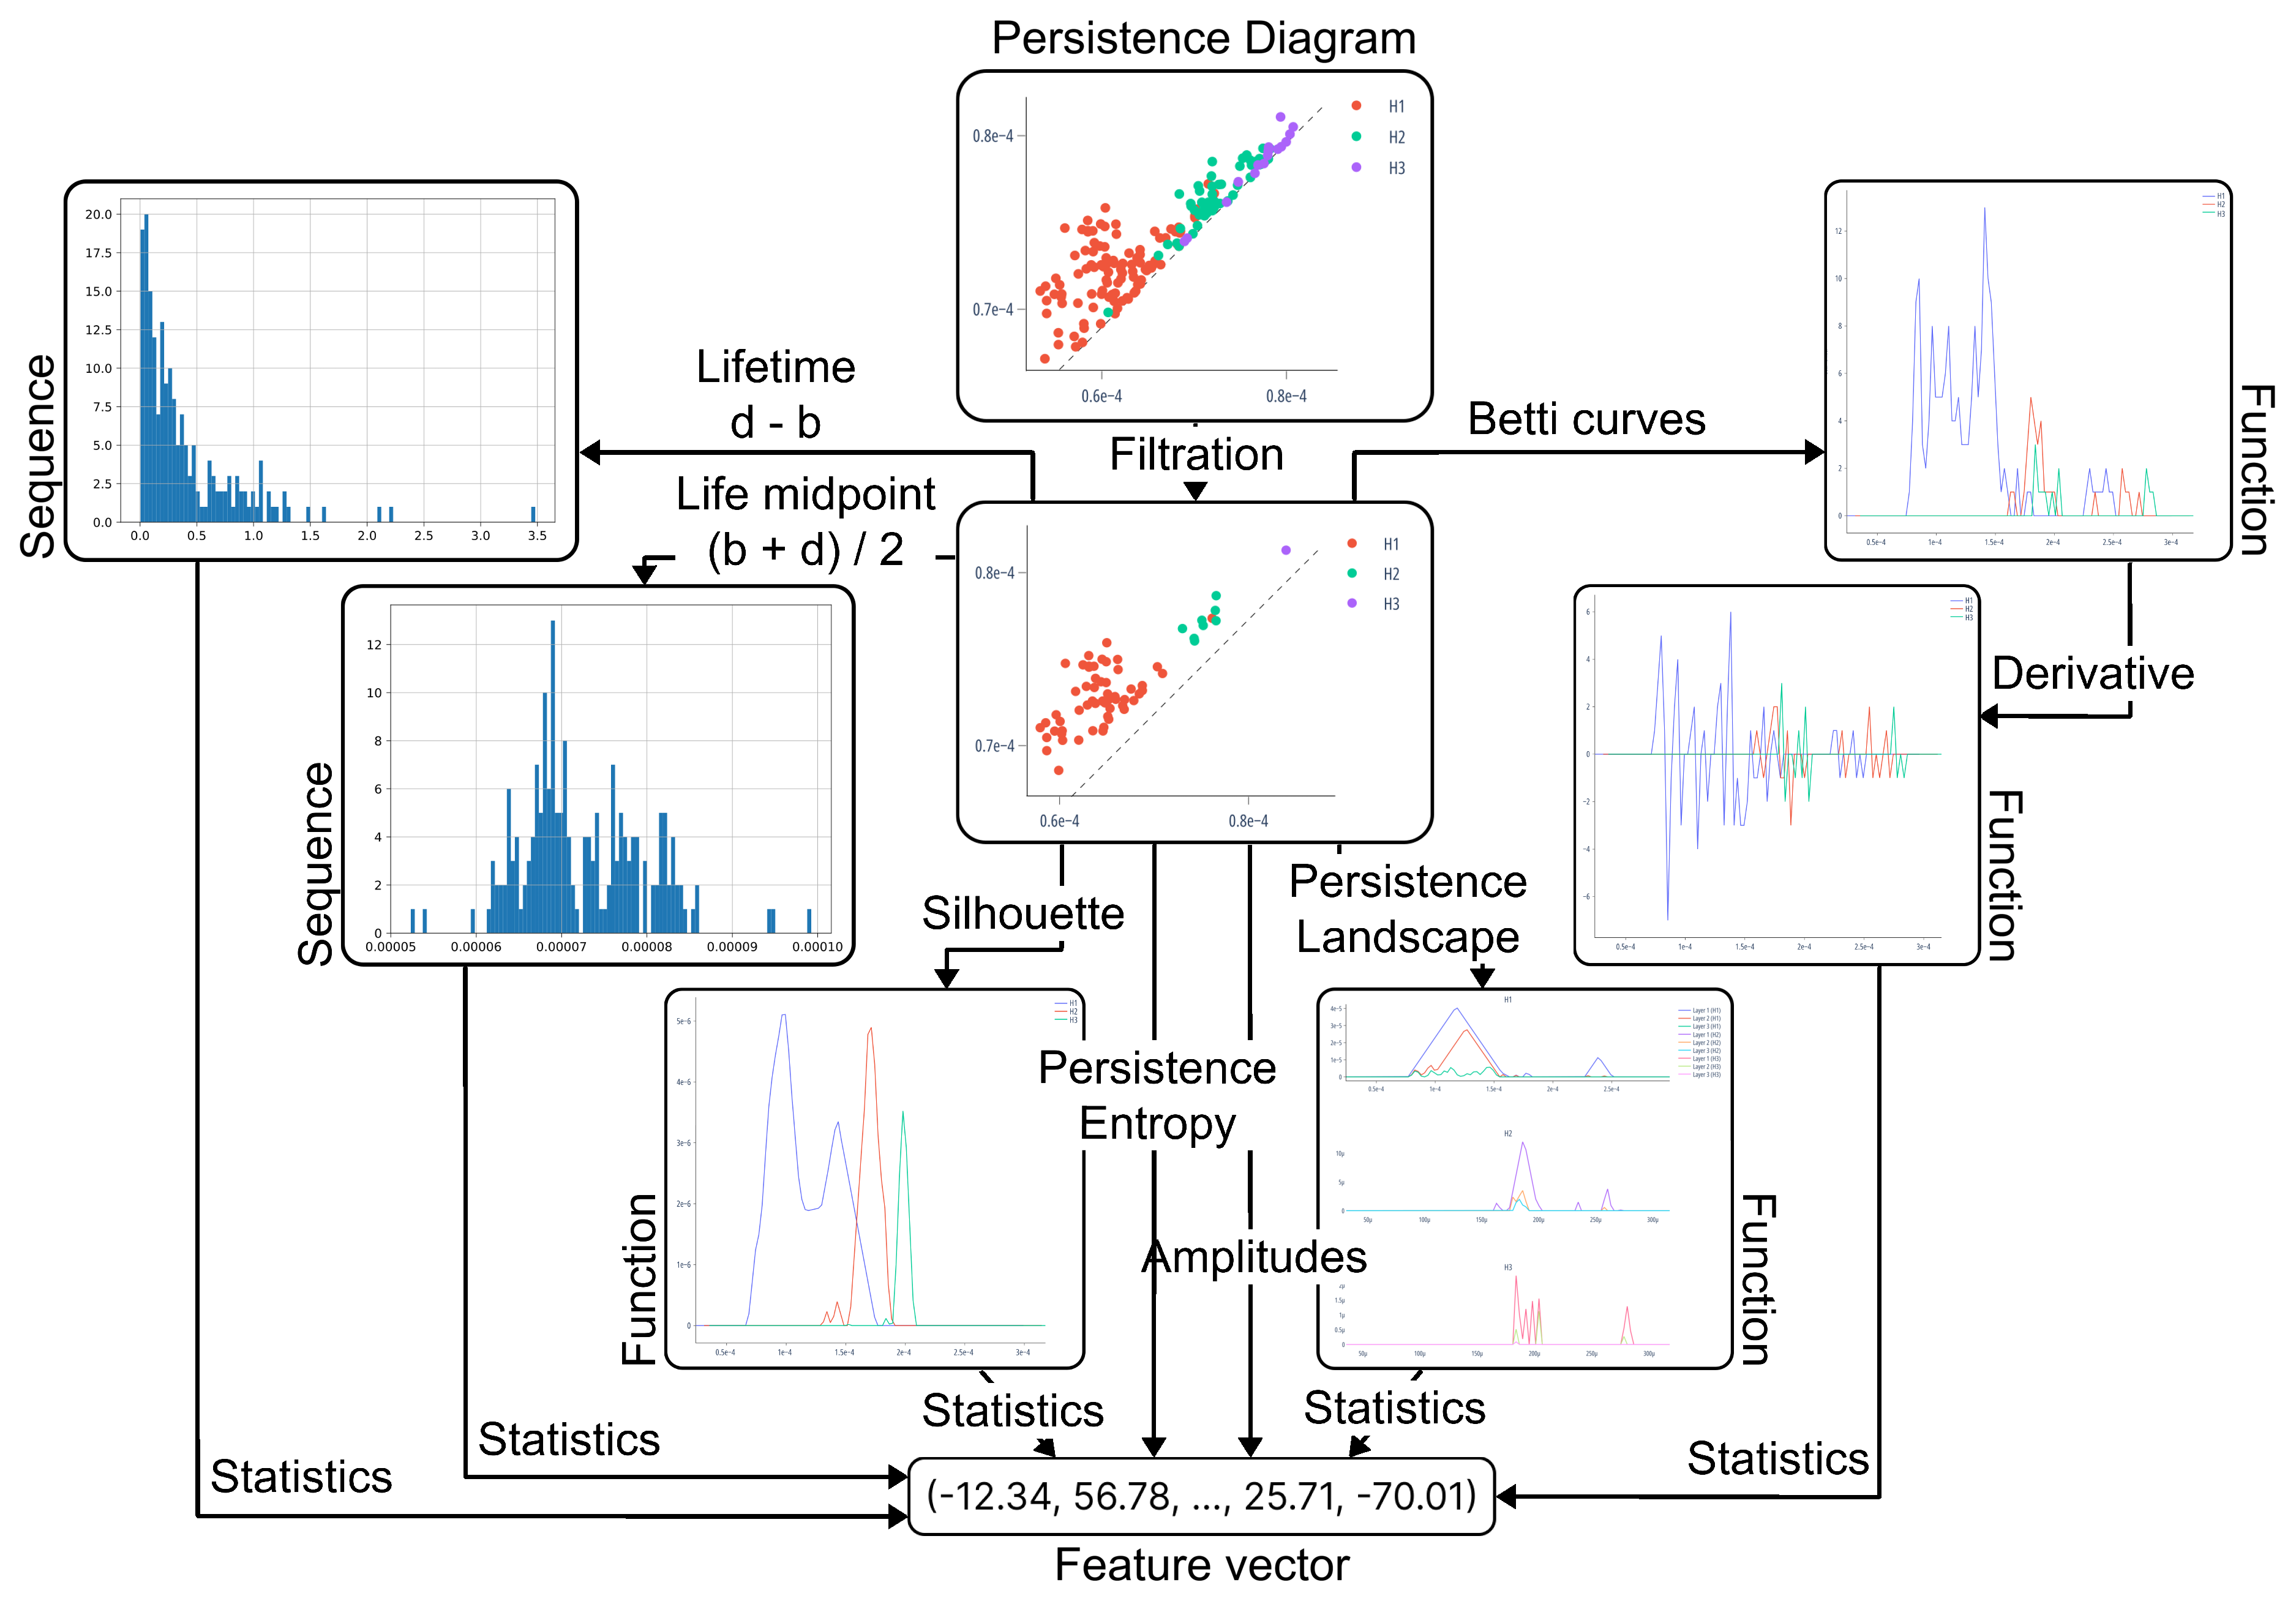
\includegraphics[width=0.65 \columnwidth]{new_Fig2.eps}
    \caption{The pipeline for vectorizing persistence diagrams. Besides the obvious, we use the first layer of persistence landscapes, persistence silhouettes of degrees 1 and 2, and amplitudes using all the aforementioned measures, as well as the bottleneck and Wasserstein distances. By the statistics of a numeric sequence or a function, that is, of a random variable, we suggest the quantity, maximum, sum, mean, standard deviation, various percentiles (25th, 50th, and 75th) of the elements, the Manhattan and Euclidean norms of the input as a vector, and the skew and kurtosis of the variable. When calculating the statistics of a function, we convert it to a numerical sequence by uniformly selecting 100 values over the interval of interest}
    \label{figure2}
\end{figure}

To improve the generalization ability of the features, the algorithm begins by filtering the persistence diagrams --- removing a fixed fraction of the points closest to the diagonal, hence representing the simplices with the shortest lifetimes. These usually carry little information and most likely describe `noise' ---  the patterns present in the original data but not generic among the objects of interest. The remaining points, in turn, are the most `long-lived' simplices that are generally most interesting for the analysis. 

The algorithm then calculates various topological and statistical characteristics described previously to construct a comprehensive feature description of the persistence diagram. To avoid missing significant patterns, we performed all calculations not only for the entire diagram but also for each simplex dimension individually. Finally, we standardize all features to remove the scale factor from further decisions, which is known to improve the quality of most machine learning methods.

\subsubsection{Feature selection}

The feature engineering algorithm described earlier is designed to detect many patterns that may be present in the analyzed time series. However, this leads to extremely high dimensionality of the resulting features, which is undesirable for most machine learning methods, including SDA, and may harm the quality of the final answer, especially if most assumed patterns are not present in the time series or appear insignificant to the target variable. To address this issue, we introduce a quick state-detecting algorithm (QSDA) --- an additional step to select the most valuable features and filter out noise that harms the final result. 

The algorithm runs a reduced SDA (that is, SDA with hyperparameters adjusted to improve performance by decreasing the number of iterations without a significant loss in quality) with only one feature, obtaining a set of state boundaries detectable with this single feature. Then, for every set of edges, we recursively generate all possible ways to reduce the number of stages by merging adjacent ones according to the rules provided by the SDA implementation, as described previously. For each said way, the algorithm estimates its quality as a multiple of the number of stages and the adapted silhouette score computed with the considered feature. This allows us to focus on the most consistently valuable features and discard those that poorly detect many stages or perfectly distinguish only a few. Finally, we define the feature quality score as the maximum of the values obtained previously, and repeat the process for all features to select the ones with the highest quality as the most informative.

One may also apply additional heuristics to remove noisy, degenerate features that score well solely because of the specifics of the approach. For example, consider a feature with only three non-zero values at indexes 300, 600, and 900 for an EEG of length 1200. In the beginning, the algorithm might calculate the boundaries $\{ 0, 280, 320, 580, 620, 880, 920, 1200 \}$, which results in a $0.74$ average silhouette and a $5.93$ final quality score of the feature, putting it above most non-degenerate ones in the end. Although the feature may contain some relevant information, it is evidently not valuable and will harm the final result. To counteract this, we preemptively filter out all features with fewer than 200 unique values --- approximately 20\% of the length of the analyzed EEG.\@

\subsubsection{Information value analysis}

Information value analysis~\cite{InformationValue} is a typical approach to evaluate the influence of individual features on the target variable in binary classification problems and can be natively generalized to assess the feature importance for clusterization.

Suppose $x=(x_1, x_2, \ldots, x_n)$ is a categorical feature with values from the set $\{ X_1, X_2, \ldots, X_k \}$. Then, the information value of this feature is computed using equation~\eqref{eq2} and is an estimate of how much the distribution of this feature coincides with the distribution of the target variable, thus showing the importance of this feature for the correct classification.
\begin{equation}
\sum_{i = 1}^{k} (sharePos_i - shareNeg_i) \cdot \ln \dfrac{sharePos_i}{shareNeg_i} \label{eq2}
\end{equation}
with:
\begin{itemize}
    \item
        $sharePos_i$ and $shareNeg_i$ are the fractions of objects in the dataset belonging to the positive and negative classes, respectively, whose value of the feature is $X_i$;
\end{itemize}

When working with quantitative features, the values are divided into several containers (we used 10) of the same length and processed as categorical based on their belonging to one or another container. For a clusterization problem, the information value is calculated as an average IV for each cluster relative to a binary indicator variable.

Large information values correspond to the high generalization ability of the feature and its significant influence on the correct prediction of the target variable. On the other hand, values close to zero indicate the harmfulness of the feature when making predictions.

\section{Results}

\subsection{Meditation data}

In this study, we primarily work with Guhyasamaja Tantra meditation data. First, we focus on subjects 1 -- 3 and compare the results obtained using 765 traditional features from~\cite{SDA}, almost 20000 topological features, a subset of 1500 -- 2000 topological features selected with QSDA, and the feature space with both approaches combined. At this stage, we determine the optimal hyperparameters, employ information value analysis, and study the scores calculated by the QSDA to select a set of approximately 4,000 topological features. The final hyperparameter values are listed in Supplementary Materials B. Then, we remove the characteristics that consistently show bad IV and QSDA quality from the computations and run the experiments for all 30 subjects to ensure the reliability of the results. To reinforce the stability of the approach, we also report the performance for noise-corrupted recordings, expecting to see no significant changes in the detected stages, and shuffled EEG epochs, anticipating the detection of no good boundaries, resulting in close-to-zero quality metrics.

\subsubsection{Full feature set for subjects~1 -- 3}

According to Fig.~\ref{figure3}, filtered topological features outperform traditional ones for all subjects and most choices of PCA components, with the combined feature space achieving an even higher adapted silhouette score for subject 1, although following slightly behind for subjects 2 and 3. Notably, for all three subjects, QSDA significantly improved the quality of the resulting edges, indicating that the technique effectively filtered out noisy, harmful features. Moreover, as expected, SDA revealed no significant patterns when applied to the shuffled recordings, demonstrating a score more than 25 times lower than that of the original data. On the contrary, adding noise had a much smaller effect, indicating that the pipeline is relatively robust with respect to noise.

Finally, we observed no obvious bifurcations in the score when changing the number of PCA components. Thus, to facilitate comparison with the original study in the following experiments, we settled on fifteen components that typically explain approximately 60--80\% of the original feature space variance, a common threshold in EEG studies. Moreover, the consistency of the results with different numbers of components confirms the statistical validity of the conclusions.

\begin{figure}
    \centering
    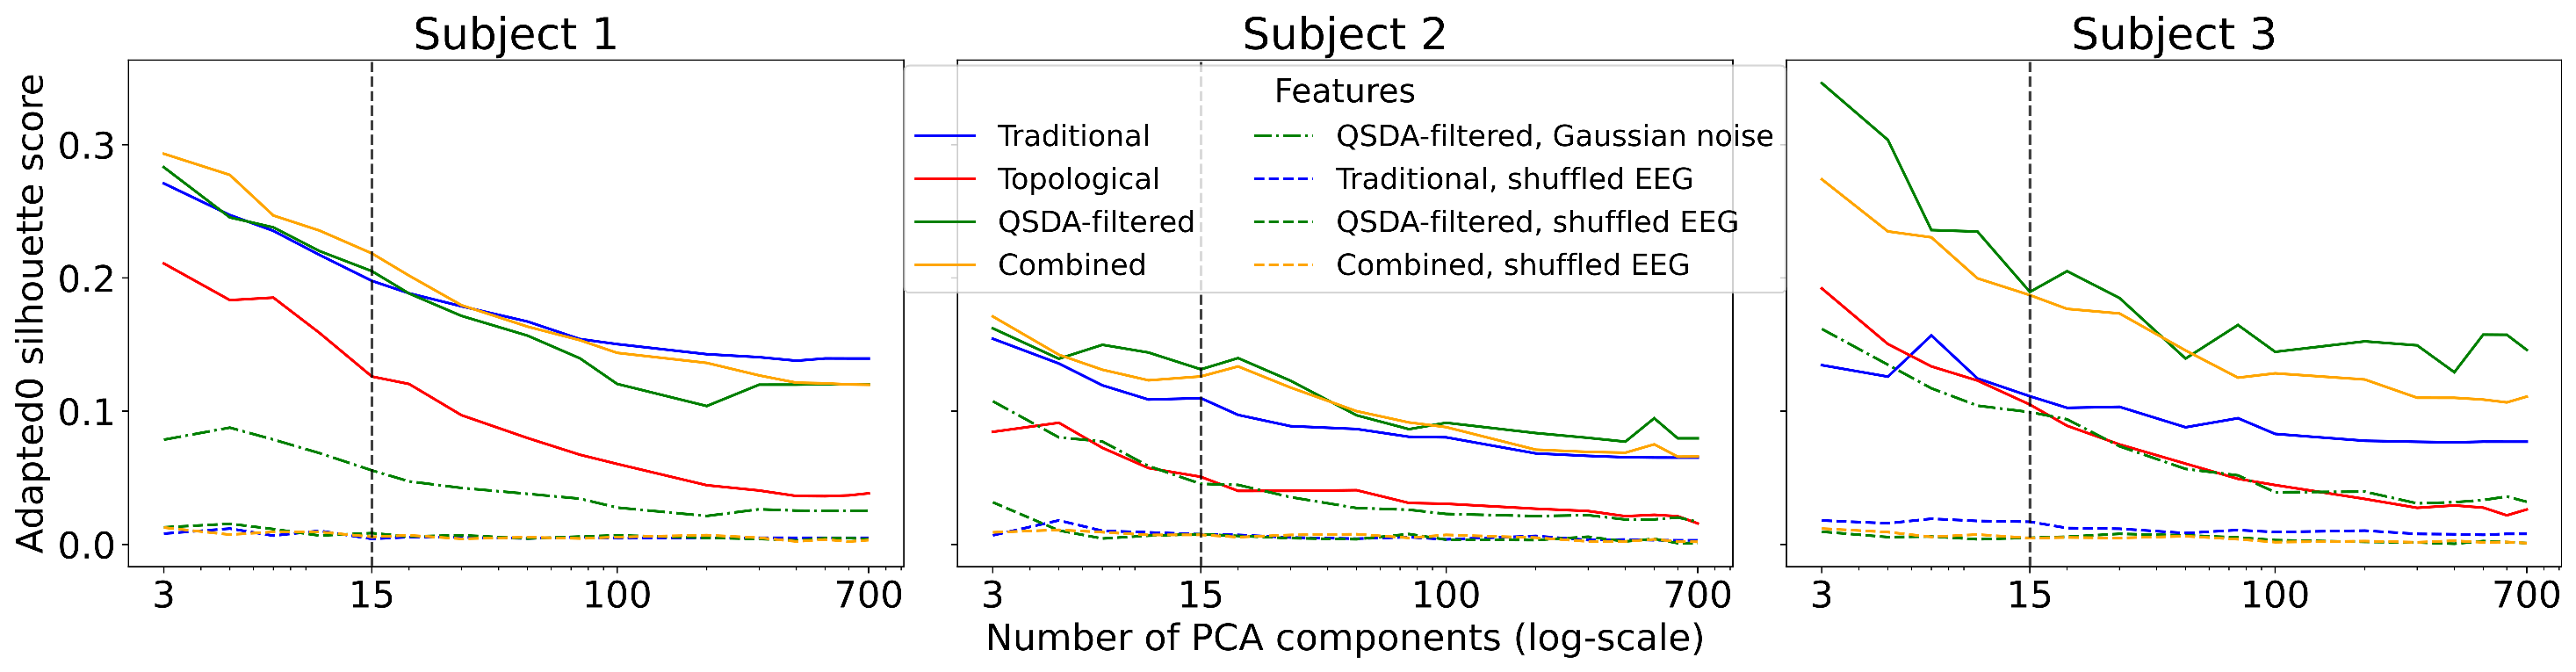
\includegraphics[width=\columnwidth]{new_Fig3.eps}
    \caption{Adapted silhouette scores of results for subjects 1 -- 3 using different sets of features with a varying number of PCA components}
    \label{figure3}
\end{figure}

Next, we review the specific results presented in Supplementary Materials C for each subject. Overall, the SDA successfully identified well-separated functional stages in all three EEG recordings for all the considered feature spaces. Although we did not achieve a complete agreement between the results, one can undoubtedly trace the common patterns confirmed by relatively good values of quality metrics.

Most importantly, topological features have demonstrated results comparable to those of traditional features, with some stage boundaries almost precisely matching across all subjects. Furthermore, the topological approach led to better partitions, as measured by the silhouette score. Traditional techniques, however, usually prevailed in terms of answer stability: the scatter plots show noticeably higher density and better separation of the stage\mbox{-}2 boundary candidates when the spectral features are involved. With topological features, the algorithm significantly shifted or did not determine the individual boundaries separating similar states with low intercluster distances. Accounting for the results with the combined feature space, we suggest that topological methods most likely do not duplicate but complement the traditional approach. Our experiments show that they may miss some critical patterns in the original data, but reveal additional significant dependencies, supported by combined features that demonstrate comparable or better quality than other approaches, while exhibiting higher stability. Finally, despite relatively low silhouette scores, the boundaries detected for noisy recordings mostly coincide with those for the original EEG, except for a few of the least stable ones, reinforcing the robustness of the topological approach.

Considering the feature quality scores presented to the right of each figure in Supplementary Materials C, QSDA and IV showed generally consistent trends. For subject 1, both strategies valued recordings from the right frontal and occipital parts; for subject 2, from the pre-frontal, frontal, and midline areas; and for subject 3, from the temporal and frontal regions. Notably, QSDA generally shifted its preference towards occipital and parietal components, although the principal trends persisted. However, neither technique revealed reliable patterns in the brain regions producing the most valuable features, indicating that no EEG channel should be excluded from further calculations. Regardless, both approaches consistently scored the features resulting from Pearson dissimilarities low.

\begin{figure}
    \centering
    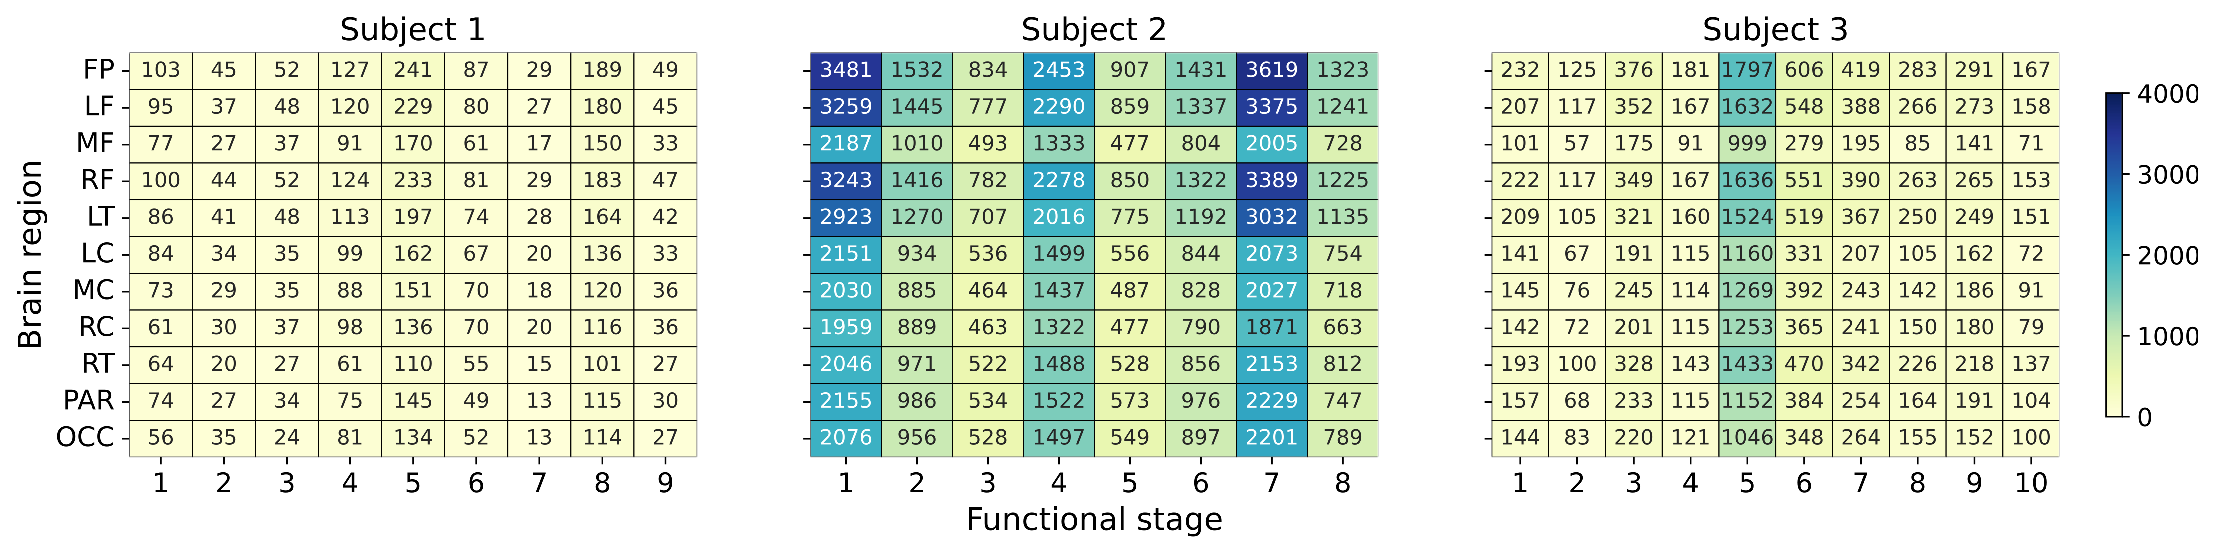
\includegraphics[width=\columnwidth]{new_Fig4.eps}
    \caption{Number of occurrences of each brain region in the dimension-5 representative cocycles, partitioned by functional stages detected with  QSDA-filtered topological features, for subjects 1 -- 3}
    \label{figure4}
\end{figure}
 
Subsequently, the most practical features, consistently across QSDA and information value analysis for all subjects, were the various persistence amplitudes. Interestingly, QSDA primarily favored those based on persistence silhouettes and landscapes, whereas those calculated from Betti curves received a higher IV.\@ Similarly, the most meaningful statistical characteristics were the vector norms, as well as the sum and mean of the sequences. The least informative, in turn, were all percentiles, skew, and kurtosis of variables. Aggregated by topological origin, although the features of dimensions 1 and 2 contributed the most, the best features were those describing all dimensions simultaneously, suggesting that higher dimensions do not duplicate but rather complement the patterns detected by simpler features.

Unexpectedly, for subject 2, QSDA also favored patterns of dimension 5, which we explore by extracting the sets of their corresponding simplices called representative cocycles. As shown in Fig.~\ref{figure4}, these features clearly distinguish stages 1, 4, and 7, with most simplex vertices located in FP, LF, RF, and LT brain regions, indicating the existence of some interactions among those neurons. Moreover, the four regions are typically considered the basis of the human brain's limbic system, an extended part of the default mode network responsible for self-referential thought, rest, emotions, and, in general, the transition between conscious and unconscious actions. Given the nature of mediation, we suggest that these features most likely detect the states of entry into and exit from meditation, supported by a reasonable correlation with the first and one of the last stages. However, no clear patterns are observed for Subject 1, and only stage 5 is detected for Subject 3, which requires further research on the physiological differences between the monks.

It is worth noting that the extremely high dimensionality of the topological features may have introduced some dispersion in the results. However, the proposed selection method (QSDA) demonstrated effectiveness in filtering out significant portions of harmful features, supported by information value analysis. Although one may notice some discrepancies in its behavior compared to IV (for example, giving preference to data collected closer to the occipital brain region and overestimating the quality of some amplitudes), the principal patterns match for both approaches.

\subsubsection{Reduced set for 30 subjects}

To speed up the subsequent computations and enhance the stability of the detected stages, we remove the consistently least effective features based on previous results: all features computed from Pearson dissimilarities; the features resulting from Betti curves and the number of points on persistence diagrams, including the respective amplitudes; the percentiles, skew, and kurtosis of the variables. By doing this, we reduce the topological feature space to approximately 4,500 features (as opposed to 20,000 previously), from which we select the 25\% best ones using QSDA. Moving forward, we repeat all the experiments for 30 subjects and report the results in Supplementary Materials D.

First, based on the silhouette scores presented in Supplementary Materials D, Table 1, and the aggregated illustration in Fig.~\ref{figure5}, topological features outperform the traditional ones for most subjects, with the combined feature spaces prevalent in a third of the recordings. Similar to previous findings, QSDA improves the results for almost all subjects, reinforcing its effectiveness in feature selection. Furthermore, Gaussian noise generally reduces the score by at most a factor of three, while shuffling the epochs drastically decreases the quality, indicating no good boundaries to be detected. Indeed, the scores in the latter case were multiple times lower than those for the original EEG and did not exceed 0.05 for most subjects. 

\begin{figure}
    \centering
    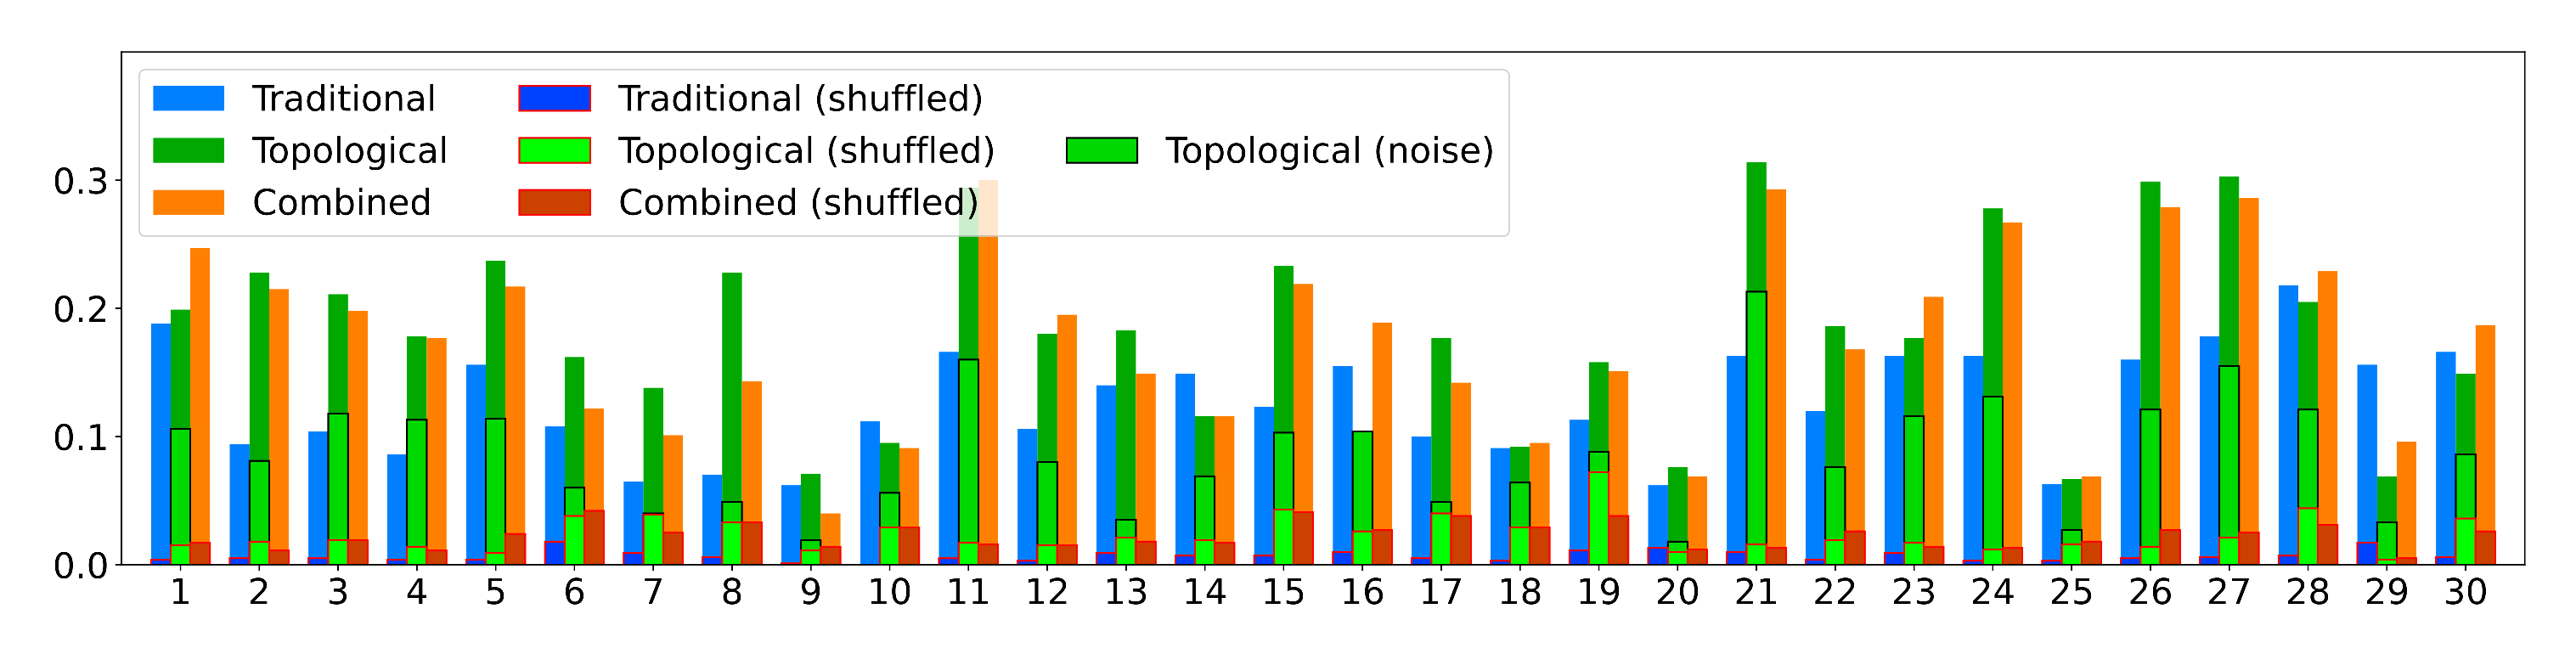
\includegraphics[width=0.9 \columnwidth]{new_Fig5.eps}
    \caption{The adapted silhouette scores of the resulting boundaries deduced by SDA using three types of features for the original and shuffled recordings of 30 subjects}
    \label{figure5}
\end{figure}

Exploring the detected stage boundaries also confirms our previous conclusions that all feature sets detect similar boundaries, with only the least stable ones noticeably shifted by the topological approach. Interestingly, the clusters derived from topological features appeared quite dense for most subjects, suggesting that the new approach is also not inferior in terms of the stability of the results. Moreover, for a significant portion of the subjects, the combined features produced more compact clusters than all other techniques, confirming that the two feature sets not only support each other but may also detect different meaningful characteristics of the EEG.

Finally, these experiments confirm which features are the most valuable for the study. As shown on the right of each figure in Supplementary Materials D, the most useful were the amplitudes, especially those based on persistence silhouettes, with the mean and sum being the most practical characteristics to consider. Interestingly, the most valuable data for the research generally comes from the electrodes in the frontal area of the brain, as confirmed by both the aggregated QSDA and IV scores in Fig.~\ref{figure6}. However, this result is not consistent across all subjects, with some exhibiting opposite tendencies, which requires further research into more specific physiological patterns of individual subjects.

\begin{figure}
    \centering
    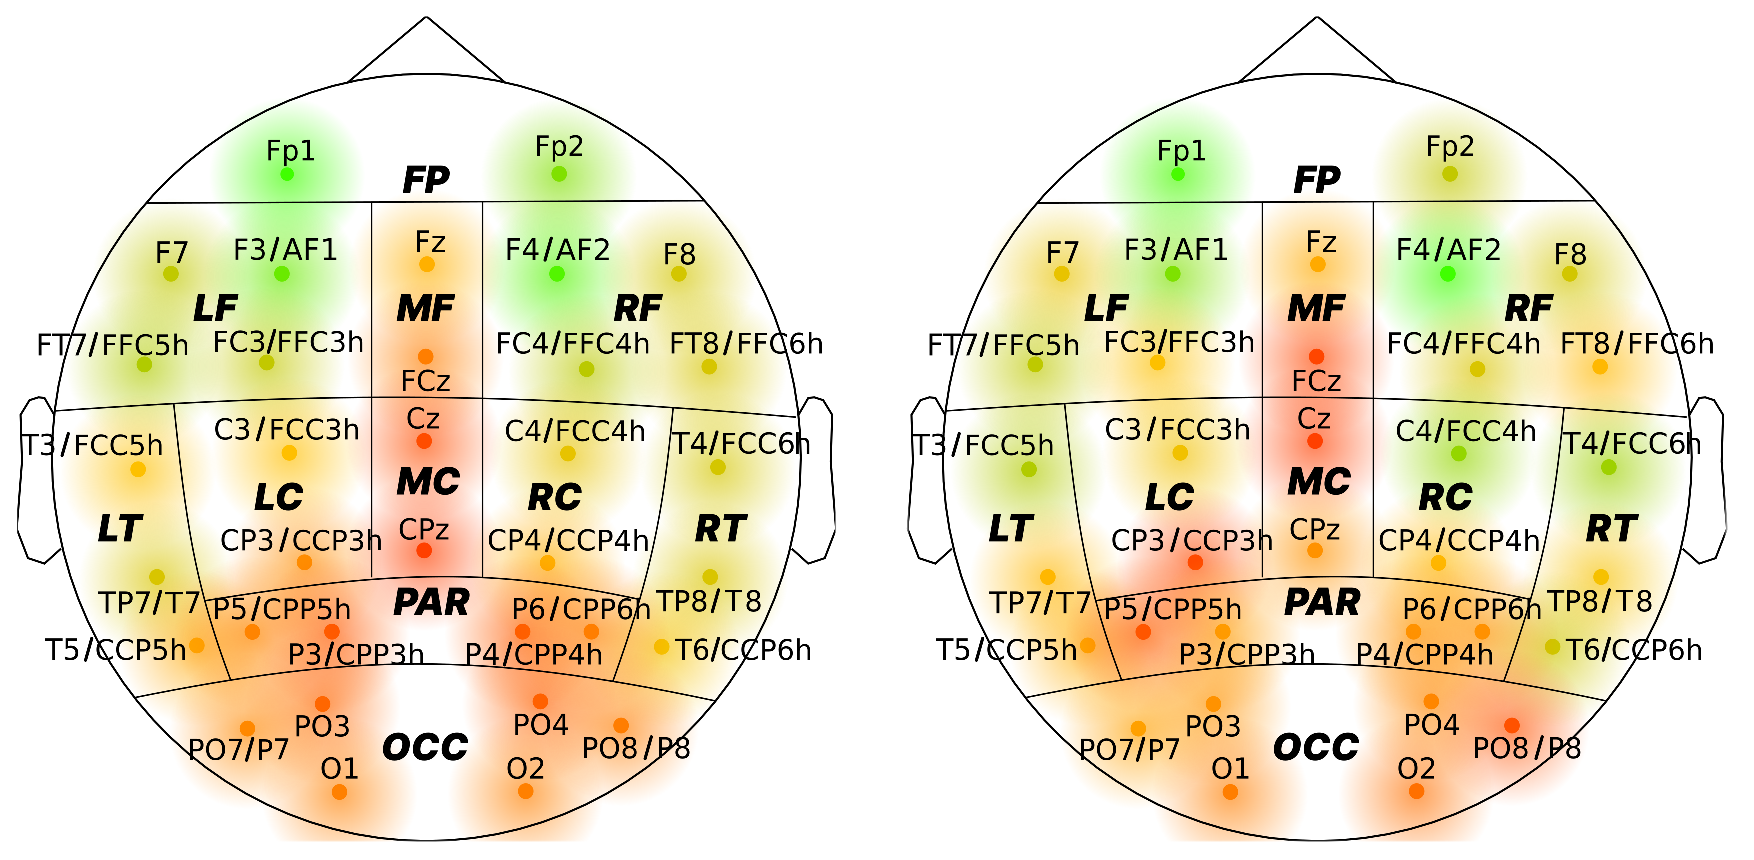
\includegraphics[width=0.6 \columnwidth]{new_Fig6.eps}
    \caption{Feature quality scores (QSDA on the left, IV on the right) aggregated by their source electrode averaged over 30 subjects. To account for the distinctions in electrode placement during different expeditions, we merge similar electrodes from different recordings into one point on the diagram. The respective mappings are indicated in the labels of such points using the `/' symbol}
    \label{figure6}
\end{figure}

Overall, the results with the full dataset confirm most patterns observed previously. Although some stages have shifted when using topological features compared to the traditional approach, general trends persist, and the method is confirmed to be robust based on its performance with noisy and shuffled recordings. Furthermore, the proposed feature selection technique demonstrated promising results, noticeably boosting the final quality and being consistent with the information value analysis. Although further research is needed to evaluate the physiological interpretation of the conclusions and to understand the reasons for the observed discrepancies, the results are sufficient to consider the proposed topological framework as an appropriate alternative to spectral features.

\subsection{Sleep data}

To reinforce our results and assess the applicability of the topological approach to other data, we run the proposed algorithm on PSG recordings from the sleep-edf~\cite{SleepEdf,PhysioNet} dataset. As mentioned previously, we search for 10 functional stages and evaluate whether they fit any subset of expert annotations. For simplicity, this section analyzes three sets of features: spectral features similar to those in \cite{SDA}, topological features, and a combination of both. Moreover, as the data contains only seven data channels, we omit the feature selection. All hyperparameters of the algorithm were left unchanged.

To assess the results, we focus on two primary quality metrics: the previously used adapted silhouette score and the Fowlkes-Mallows index (FMI)~\cite{Fowlkes01091983}. The latter is a typical external criterion used to measure the degree of similarity between two clusterings. For a predicted set of stage boundaries $A = (a_1, a_2, \dots, a_n)$ and an expert annotation $E = (e_1, e_2, \dots, e_m)$, we select a subset $F = (f_1, f_2, \dots, f_n) \subset E$ of boundaries with the lowest sum of pairwise distances to A ($\sum_{i = 1}^{n} |a_i - f_i| \rightarrow \min$) and determine whether their `true' cluster distribution matches the predicted one by computing the FMI according to equation~\eqref{eq3}.
\begin{equation}
    FMI = \sqrt{\frac{TP}{TP + FP} \cdot \frac{TP}{TP + FN}} \label{eq3}
\end{equation}
with:
\begin{itemize}
    \item
        $TP$ the number of pairs of epochs assigned to the same cluster in both distributions;
    \item
        $FP$ --- same cluster in the `true' distribution, different clusters in the predicted one;
    \item
        $FN$ --- same cluster in the predicted distribution, different clusters in the `true' one.
\end{itemize}

Interestingly, the topological approach appeared noticeably superior to the traditional features for this data in both the silhouette score and the FMI.\@ As shown in Table~\ref{table1}, the average adapted silhouette among the 153 subjects emerged over seven times better for topological features than traditional ones, with the predictions resembling expert annotations on average 8\% better, as indicated by the FMI. Moreover, the confidence intervals of both metrics for both feature sets are remarkably small and, most importantly, do not overlap with each other, confirming the statistical significance of the results. Furthermore, a similar or arguably slightly worse quality obtained with the combined feature space suggests that the topological approach supersedes traditional features, revealing not only new patterns but also supporting the already known ones.


\begin{table}
\caption{Mean quality scores and their 95\% confidence intervals of results for sleep data of 153 subjects}
\label{table1}
\begin{tabular}{cccc}
  \toprule
    Feature set & Adapted silhouette & Fowlkes-Mallows index \\
  \midrule
    Traditional & $0.03 \pm 0.009$  & $0.843 \pm 0.017$ \\
    Topological & $0.228 \pm 0.01 $ & $0.911 \pm 0.013$ \\
    Combined &  $0.227 \pm 0.01 $ & $0.907 \pm 0.014$ \\
  \bottomrule
\end{tabular}
\end{table}

Next, we present the comprehensive results separately for each subject in Supplementary Materials E. The figures suggest that all feature sets generally detect similar stages. Notably, the final boundaries typically fall within tight groups of expert labels, indicating that the algorithm effectively finds high-level clusterings, and the limitation of 10 searched stages does not impact the interpretability of the results. Moreover, as suggested by the densities of the scatter plots, topological features produce significantly more robust results, which at the same time better correspond to target labelings. The quality score diagrams at the beginning of Supplementary Materials E also support the findings that traditional features consistently perform worse than the topological approach in terms of both stability and agreement with target answers.

Overall, the results for sleep-edf reflect previous findings from the meditation data but strongly suggest the superiority of the topological approach. Despite searching for only ten stages, our experiments show that with topological features, SDA consistently produces more robust boundaries that better match the target distribution, even without feature selection.\@

\section{Discussion}

In this study, we propose a novel feature engineering pipeline for EEG segmentation based on topological data analysis, aiming to capture the geometry and spatial characteristics of the data. Our experiments suggest that the technique produces similar boundaries to the traditional approach for Guhyasamaja Tantra meditation, and the resulting stage boundaries are significantly more consistent with expert annotations for the sleep-edf dataset. Moreover, the results obtained with noisy and shuffled data confirm the technique's robustness, ensuring that the topological approach is a trustworthy alternative to traditional methods. Nonetheless, we suggest that neither approach extracts a complete description of the EEG in the general case. In practice, one should combine the techniques to capture all aspects of the data and obtain a robust outcome.

Additionally, we introduced QSDA, an SDA-based feature selection framework tailored to the final task and scalable to large feature sets. We demonstrated that QSDA effectively removes harmful features and its scores generally correlate with information values, reinforcing the robustness of the method. Furthermore, using QSDA, we identified that the most valuable features for Guhyasamaja Tantra meditation data generally come from sensors in the frontal areas of the brain. Although we do not currently have an explanation for this phenomenon, it is an interesting observation that may lead to important physiological conclusions.

Considering the large size of the topological feature space, it is essential to assess whether the gains in the quality of the final answer justify the computational expenses of generating so many features. Since estimating the theoretical complexity of such an elaborate pipeline is infeasible, we resort to an empirical analysis of the running times using samples from both datasets, ranging from 50 to 500 epochs. As shown in Fig.~\ref{figure7}, calculating the topological features is indeed more expensive than the traditional ones for both datasets. However, the difference is not as significant as one might expect, and the topological approach may have potential for optimization in the future, given the novelty of TDA. Therefore, the proposed framework is a practical alternative to traditional features showing similar and, arguably, even better results with reasonable losses in computational efficiency.

\begin{figure}
    \centering
    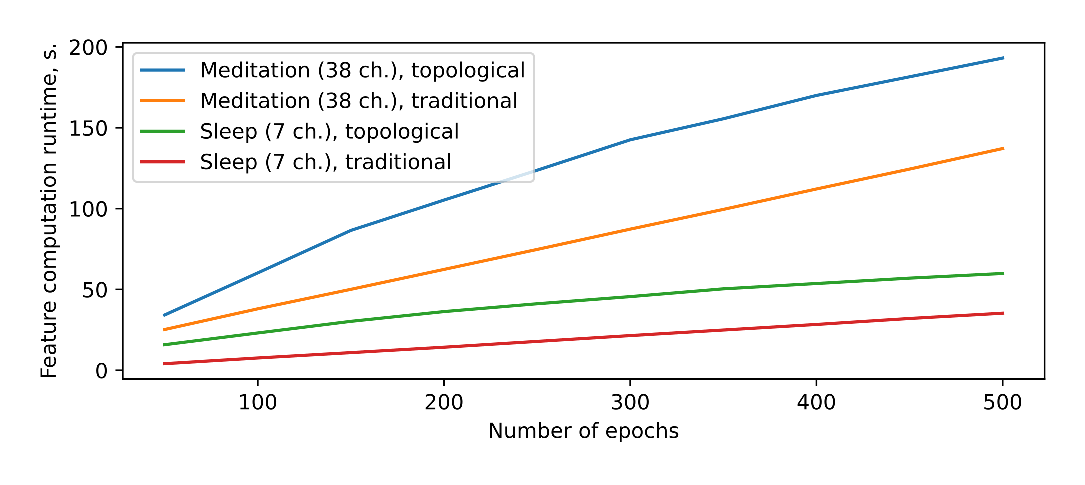
\includegraphics[width=0.7 \columnwidth]{new_Fig7.eps}
    \caption{The running time of calculating traditional and topological features for two types of data, depending on the number of epochs. Each point is an average of 25 measurements. The 95\% confidence intervals for each entry do not exceed 1\% of their absolute value}
    \label{figure7}
\end{figure}

Future studies should test the proposed approach with other datasets to collect more examples, generalize the technique, and identify common patterns. Moreover, we anticipate significant results from studies aimed at interpreting the patterns recorded by topological features, accounting for prior physiological knowledge.

\section{Conclusion}

Overall, this study provides a robust feature engineering approach for time series data, which has proved to be an effective alternative to spectral features for EEG segmentation using SDA, as confirmed by similar or even superior results with two different datasets. We believe that exploring the inherent interpretability of the approach may lead to interesting physiological conclusions, and we are confident that the proposed framework is applicable far beyond the scope of EEG.

Additionally, we present QSDA, an SDA-based task-specific feature selection technique, which we used to identify that the most valuable features for meditation data generally come from electrodes located in the frontal areas of the brain. Although the study primarily focuses on the engineering part of the task, we consider this an interesting observation worthy of consideration by physiological experts.

\section*{Declarations}

\subparagraph{\textbf{Data availability}}
The raw data will be made available by the authors upon request, without undue reservation.

\subparagraph{\textbf{Ethics approval and consent to participate}}
The studies involving humans were approved by Moscow State University. The studies were conducted in accordance with the Declaration of Helsinki, the local legislation and institutional requirements. All participants provided written informed consent to participate in this study.

\subparagraph{\textbf{Competing interests}}
The authors declare no competing interests.

\subparagraph{\textbf{Acknowledgment}}
This study was supported by the Russian Science Foundation, Grant No. 24-68-00030.

\bibliography{new_references}

\subparagraph{\textbf{Abramov Aleksandr}} Data science and software engineering master student at HSE University, Faculty of Computer Science.
\subparagraph{\textbf{Ekaterina Mikhaylets}} Associate professor at HSE University with a PhD in Discrete Mathematics and Mathematical Cybernetics.
\subparagraph{\textbf{Vsevolod Chernyshev}} Researcher at Ulm University with a PhD in Geometry and Topology.
\subparagraph{\textbf{Alexander Kaplan}} PhD and D.Sc in neurophysiology and psychophysiology from the Lomonosov Moscow State University, Professor Head of the Laboratory for Neurophysiology and Neuro-Computer Interfaces.
\subparagraph{\textbf{Fedor Ratnikov}} PhD, associate professor at HSE University, Leading Researcher at the Laboratory of Methods for Big Data Analysis.

\end{document}
